\subsection{Properties of the class associated with an exact sequence}

PROPOSITION 3. — Let

\begin{enumerate}
\def\labelenumi{(\arabic{enumi})}
\setcounter{enumi}{5}
\tightlist
\item
\end{enumerate}

\[
0 \rightarrow \mathrm{P} \rightarrow \mathrm{S} _ {m} \rightarrow \mathrm{S} _ {m - 1} \rightarrow \dots \rightarrow \mathrm{S} _ {1} \stackrel {\lambda_ {n}} {\rightarrow} \mathrm{N} \rightarrow 0\tag{7}
\]

\[
0 \rightarrow \mathrm{N} \xrightarrow {\mu} \mathrm{R} _ {n} \rightarrow \mathrm{R} _ {n - 1} \rightarrow \dots \rightarrow \mathrm{R} _ {1} \rightarrow \mathrm{M} \rightarrow 0
\]

two exact sequences of left A-modules of respective classes \(\theta\in\mathrm{Ext}_{\mathbf{A}}^{m}(\mathbf{N},\mathbf{P})\) and \(\theta^{\prime}\in\mathrm{Ext}_{\mathbf{A}}^{n}(\mathbf{M},\mathbf{N})\) . The class in \(\mathrm{Ext}_{\mathbf{A}}^{m+n}(\mathbf{M},\mathbf{P})\) associated with the exact sequence

\[
0 \to \mathrm{P} \to \mathrm{S} _ {m} \to \dots \to \mathrm{S} _ {1} \xrightarrow {\mu \circ \lambda} \mathrm{R} _ {n} \to \dots \to \mathrm{R} _ {1} \to \mathrm{M} \to 0\tag{8}
\]

is the composition product \(\theta\circ\theta'\) .

Let us choose commutative diagrams

\[
\begin{array}{c} 0 \longrightarrow \mathrm{P} \longrightarrow \mathrm{I} ^ {0} (\mathrm{P}) \longrightarrow \dots \longrightarrow \mathrm{I} ^ {m - 1} (\mathrm{P}) \xrightarrow {\delta_ {\mathrm{P}} ^ {m - 1}} \mathrm{I} ^ {m} (\mathrm{P}) \\ 0 \longrightarrow \mathrm{P} \longrightarrow \mathrm{S} _ {m} \longrightarrow \dots \longrightarrow \mathrm{S} _ {1} \xrightarrow {\lambda} \mathrm{N} \longrightarrow 0, \end{array}
\]

\[
\begin{array}{c c c c c c c c c c c c} 0 \longrightarrow & \mathrm{N} & \stackrel {{e _ {\mathrm{N}}}} {{\longrightarrow}} & \mathrm{I} ^ {0} (\mathrm{N}) & \longrightarrow & \dots & \longrightarrow & \mathrm{I} ^ {n - 1} (\mathrm{N}) & \longrightarrow & \mathrm{I} ^ {n} (\mathrm{N}) \\ & \uparrow_ {1 _ {\mathrm{N}}} & & v ^ {0} \uparrow & & & & v ^ {n - 1} \uparrow & & v ^ {n} \uparrow \\ 0 \longrightarrow & \mathrm{N} & \stackrel {{\mu}} {{\longrightarrow}} & \mathrm{R} _ {n} & \longrightarrow & \dots & \longrightarrow & \mathrm{R} _ {1} & \longrightarrow & \mathrm{M} & \longrightarrow & 0. \end{array}
\]

Since \(\mathrm{I}^{m}(\mathrm{P})\) is injective, there exists a homomorphism \(h^{0}: \mathrm{I}^{0}(\mathrm{N}) \to \mathrm{I}^{m}(\mathrm{P})\) such that \(w^{m} = h^{0} \circ e_{N}\) ; by X, p.~49, prop. 3 bis, \(h^{0}\) extends to a morphism of complexes \(h: \mathrm{I}(\mathrm{N}) \to \mathrm{I}(\mathrm{P})(-m)\) . Then \(w^{m} = h^{0} \circ e_{N} = h^{0} \circ v^{0} \circ \mu\) , hence

\[
\delta_ {1} ^ {m - 1} \circ w ^ {m - 1} = w ^ {m} \circ \lambda = h ^ {0} \circ v ^ {0} \circ (\mu \circ \lambda),
\]

and the following diagram is commutative:

\[
\begin{array}{l}0 \longrightarrow \mathrm{P} \longrightarrow \mathrm{I} ^ {0} (\mathrm{P}) \longrightarrow \dots \longrightarrow \mathrm{I} ^ {m - 1} (\mathrm{P}) \longrightarrow \mathrm{I} ^ {m} (\mathrm{P}) \longrightarrow \mathrm{I} ^ {m + 1} (\mathrm{P}) \longrightarrow \dots \longrightarrow \mathrm{I} ^ {m + n} (\mathrm{P})\\0 \longrightarrow \mathrm{P} \longrightarrow \mathrm{S} _ {m} \longrightarrow \dots \longrightarrow \mathrm{S} _ {1} \underset {\mu \circ \lambda} {\longrightarrow} \mathrm{R} _ {n} \longrightarrow \mathrm{R} _ {n - 1} \longrightarrow \dots \longrightarrow \mathrm{M} \rightarrow 0\end{array}
\]

where \(t^0 = h^0 \circ v^0\) , \(t^1 = (-1)^m h^1 \circ v^1, \ldots, t^i = (-1)^{mi} h^i \circ v^i, \ldots, t^n = (-1)^{mn} h^n \circ v^n\) . The class \(\theta\) associated with (6) is that of \((-1)^{m(m+1)/2} w^m \in \text{Homgr}_A^m(\mathbf{N}, \mathbf{l}(\mathbf{P}))\) , hence corresponds under the isomorphism \(a_{\mathbf{N},\mathbf{P}}\) to the class of \((-1)^{m(m+1)/2} h \in \text{Homgr}_A^m(\mathbf{l}(\mathbf{N}), \mathbf{l}(\mathbf{P}))\) ; the class \(\theta'\) associated with (7) is that of \((-1)^{n(n+1)/2} v^n \in \text{Homgr}_A^m(\mathbf{M}, \mathbf{l}(\mathbf{N}))\) , the class associated with (8) is that of \((-1)^{(m+n)(m+n+1)/2} t^n \in \text{Homgr}_{m+n}^m(\mathbf{M}, \mathbf{l}(\mathbf{P}))\) whence the conclusion, by the definition of the composition product (X, p.~114) and the formula

\[
m (m + 1) / 2 + n (n + 1) / 2 = (m + n) (m + n + 1) / 2 - m n.
\]

\begin{enumerate}
\def\labelenumi{\arabic{enumi}.}
\setcounter{enumi}{3}
\tightlist
\item
  --- Consider a commutative diagram of A-modules with exact
\end{enumerate}

rows

\pandocbounded{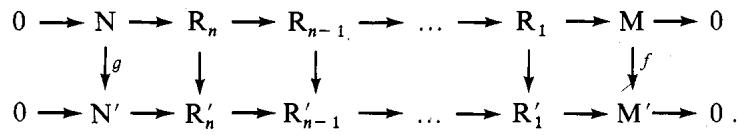
\includegraphics[keepaspectratio]{images/part001_b790ce53.jpg}}

Let θ (resp. θ′) be the class of the first (resp. second) row in

\[
\operatorname{Ext} _ {\mathbf {A}} ^ {n} (\mathbf {M}, \mathbf {N}) \quad \left(\text { resp.   } \operatorname{Ext} _ {\mathbf {A}} ^ {n} (\mathbf {M} ^ {\prime}, \mathbf {N} ^ {\prime})\right).
\]

In \(\operatorname{Ext}_{\mathbf{A}}^{n}(\mathbf{M}, \mathbf{N}')\) , one has \(\theta' \circ f = g \circ \theta\) .

Indeed, consider a commutative diagram

\pandocbounded{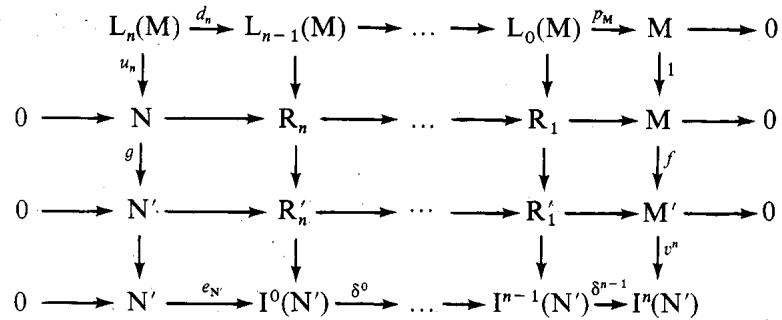
\includegraphics[keepaspectratio]{images/part001_126cf8d3.jpg}}

By definition \(\theta' \circ f\) is the class of \((-1)^{n(n+1)/2} v^n \circ f \circ p_M \in \text{Homgr}^n (\text{L(M)}, \text{I(N')})\) , whereas \(g \circ \theta\) is the class of \((-1)^{n(n+1)/2} e_{N'} \circ g \circ u_n\) . By Lemma 1, applied to the two extreme rows of the diagram, these two classes are equal.

COROLLARY 1. --- Consider a commutative diagram with exact rows

\[
\begin{array}{c c c c c c c c} 0 \longrightarrow & \mathrm{N} \longrightarrow & \mathrm{R} _ {n} \longrightarrow & \dots & \longrightarrow & \mathrm{R} _ {1} \longrightarrow & \mathrm{M} \longrightarrow & 0 \\ & ^ {1} \downarrow & & & \downarrow & & ^ {1} \downarrow \\ 0 \longrightarrow & \mathrm{N} \longrightarrow & \mathrm{R} _ {n} ^ {\prime} \longrightarrow & \dots & \longrightarrow & \mathrm{R} _ {1} ^ {\prime} \longrightarrow & \mathrm{M} \longrightarrow & 0; \end{array}
\]

the two rows of the diagram have the same associated class in \(\operatorname{Ext}_{\mathbf{A}}^{n}(\mathbf{M},\mathbf{N})\) .

COROLLARY 2. --- Let

\[
0 \rightarrow \mathrm{N} \xrightarrow {f _ {n - 1}} \mathrm{R} _ {n} \xrightarrow {f _ {n}} \mathrm{R} _ {n - 1} \rightarrow \dots \xrightarrow {f _ {2}} \mathrm{R} _ {1} \xrightarrow {f _ {1}} \mathrm{M} \rightarrow 0
\]

be an exact sequence, \(\theta\in\mathrm{Ext}_{\mathbf{A}}^{n}(\mathbf{M},\mathbf{N})\) the associated class, \(a_{1},\ldots,a_{n+1}\) invertible elements of \(k\) . The class associated with the exact sequence

\[
0 \rightarrow \mathrm{N} \xrightarrow {a _ {n + 1} f _ {n + 1}} \mathrm{R} _ {n} \xrightarrow {a _ {n} f _ {n}} \mathrm{R} _ {n - 1} \rightarrow \dots \xrightarrow {a _ {2} f _ {2}} \mathrm{R} _ {1} \xrightarrow {a _ {1} f _ {1}} \mathrm{M} \rightarrow 0
\]

is \((a_{1}^{-1}a_{2}^{-1}\dots a_{n + 1}^{-1})\theta .\)

Indeed, we have a commutative diagram

\[
\begin{array}{c} 0 \longrightarrow \mathrm{N} \xrightarrow {a _ {n + 1} f _ {n + 1}} \mathrm{R} _ {n} \longrightarrow \dots \longrightarrow \mathrm{R} _ {2} \xrightarrow {a _ {2} f _ {2}} \mathrm{R} _ {1} \xrightarrow {a _ {1} f _ {1}} \mathrm{M} \longrightarrow 0 \\ \Biggl \downarrow a _ {1} \dots a _ {n + 1} \quad \Biggl \downarrow a _ {1} \dots a _ {n} \quad \Biggl \downarrow a _ {1} a _ {2} \quad \Biggl \downarrow a _ {1} \quad \Biggl \downarrow 1 \\ 0 \longrightarrow \mathrm{N} \xrightarrow {f _ {n + 1}} \mathrm{R} _ {n} \longrightarrow \dots \longrightarrow \mathrm{R} _ {2} \xrightarrow {f _ {2}} \mathrm{R} _ {1} \xrightarrow {f _ {1}} \mathrm{M} \longrightarrow 0. \end{array}
\]

and we apply the proposition.

COROLLARY 3. --- Let \(0 \to \mathbf{N} \xrightarrow{f_{n+1}} \mathbf{R}_{n} \xrightarrow{f_{n}} \cdots \to \mathbf{R}_{1} \xrightarrow{f_{1}} \mathbf{M} \to 0\) be an exact sequence, \(\theta\) its class in \(\operatorname{Ext}_{\mathbf{A}}^{n}(\mathbf{M}, \mathbf{N})\) , \(u: \mathbf{M}' \to \mathbf{M}\) and \(v: \mathbf{N} \to \mathbf{N}'\) be two homomorphisms of A-modules.

\begin{enumerate}
\def\labelenumi{\alph{enumi})}
\tightlist
\item
  The element \(v \circ \theta\) of \(\operatorname{Ext}_{\mathbf{A}}^{n}(\mathbf{M}, \mathbf{N}')\) is equal to the class of the exact sequence
\end{enumerate}

\[
0 \rightarrow \mathrm{N} ^ {\prime} \xrightarrow {f _ {n + 1} ^ {\prime}} \mathrm{R} _ {n} ^ {\prime} \xrightarrow {f _ {n} ^ {\prime}} \mathrm{R} _ {n - 1} \xrightarrow {f _ {n - 1}} \dots \rightarrow \mathrm{R} _ {1} \rightarrow \mathrm{M} \rightarrow 0,
\]

where \(R_{n}^{\prime}\) is the A-module quotient of \(R_{n} \oplus N^{\prime}\) by the submodule formed by the pairs \((f_{n+1}(x), -v(x))\) for \(x \in N\) , and where \(f_{n+1}^{\prime}\) (resp. \(f_{n}^{\prime}\) ) is deduced from the canonical injection (resp. from \((f_{n}, 0)\) ) by passing to quotients.

\begin{enumerate}
\def\labelenumi{\alph{enumi})}
\setcounter{enumi}{1}
\tightlist
\item
  The element \(\theta \circ u\) of \(\operatorname{Ext}_{\mathbf{A}}^{n}(\mathbf{M}^{\prime}, \mathbf{N})\) is the class of the exact sequence
\end{enumerate}

\[
0 \rightarrow \mathrm{N} \rightarrow \mathrm{R} _ {n} \rightarrow \dots \rightarrow \mathrm{R} _ {2} \xrightarrow {f _ {2} ^ {\prime \prime}} \mathrm{R} _ {1} ^ {\prime} \xrightarrow {f _ {1} ^ {\prime \prime}} \mathrm{M} ^ {\prime} \rightarrow 0,
\]

where \(R_{1}^{\prime}\) is the fiber product \(R_{1} \times_{M} M^{\prime}\) , that is to say (I, p.~44) the submodule of \(R_{1} \times M^{\prime}\) formed by the pairs \((x, y)\) such that \(f_{1}(x) = u(y)\) , and where \(f_{2}^{\prime\prime}\) (resp. \(f_{1}^{\prime\prime}\) ) is deduced from \((f_{2}, 0)\) (resp. from the second projection).

Let us prove for example \(a\) ). Let \(z\) be an element of \(\mathbf{R}_{n}^{\prime}\) such that \(f_{n}^{\prime}(z)=0\) ; if \(z\) is the class of a pair \((x,y)\) , with \(x\in\mathbf{R}_{n},y\in\mathbf{N}^{\prime}\) , we have \(f_{n}(x)=0\) so that there exists an element \(t\in\mathbf{N}\) such that \(x=f_{n+1}(t)\) . We then have \(z=f_{n+1}^{\prime}(y+v(t))\) which proves that \(\operatorname{Ker} f_{n}^{\prime}=\operatorname{Im} f_{n+1}^{\prime}\) . The injectivity of \(f_{n+1}^{\prime}\) follows from that of the \(f_{n+1}\) .

Let \(j: \mathbf{R}_{n} \to \mathbf{R}_{n}^{\prime}\) be the homomorphism deduced from the canonical injection; we have a commutative diagram of exact sequences:

\[
\begin{array}{c} 0 \longrightarrow \mathrm{N} \xrightarrow {f _ {n + 1}} \mathrm{R} _ {n} \xrightarrow {f _ {n}} \mathrm{R} _ {n - 1} \longrightarrow \dots \longrightarrow \mathrm{M} \longrightarrow 0 \\ \Biggl \downarrow v \quad \Biggl \downarrow j \quad \Biggl \downarrow 1 \\ 0 \longrightarrow \mathrm{N} ^ {\prime} \xrightarrow {f _ {n + 1} ^ {\prime}} \mathrm{R} _ {n} ^ {\prime} \xrightarrow {f _ {n} ^ {\prime}} \mathrm{R} _ {n - 1} \longrightarrow \dots \longrightarrow \mathrm{M} \longrightarrow 0; \end{array}
\]

assertion a) then follows from the proposition.

The proof of \(b\) is analogous.

Remark. --- Let \(\theta\in\mathrm{Ext}_{\mathbf{A}}^{n}(\mathbf{M},\mathbf{N})\) , resp. \(\theta^{\prime}\in\mathrm{Ext}_{\mathbf{A}}^{n}(\mathbf{M}^{\prime},\mathbf{N}^{\prime})\) , be the class of an exact sequence

\[
0 \rightarrow \mathrm{N} \xrightarrow {f _ {n + 1}} \mathrm{R} _ {n} \rightarrow \dots \rightarrow \mathrm{R} _ {1} \xrightarrow {f _ {1}} \mathrm{M} \rightarrow 0,
\]

\[
\text { resp. } 0 \to \mathrm{N} ^ {\prime} \xrightarrow {f _ {n + 1} ^ {\prime}} \mathrm{R} _ {n} ^ {\prime} \to \dots \to \mathrm{R} _ {1} ^ {\prime} \xrightarrow {f _ {1} ^ {\prime}} \mathrm{M} ^ {\prime} \to 0.
\]

Let \(i_{\mathbf{N}}, i_{\mathbf{N}'}\) , be the canonical injections of \(\mathbf{N}\) and \(\mathbf{N}'\) into \(\mathbf{N} \oplus \mathbf{N}'\) , \(q_{\mathbf{M}}\) , \(q_{\mathbf{M}'}\) , the projections of \(\mathbf{M} \oplus \mathbf{M}'\) onto \(\mathbf{M}\) and \(\mathbf{M}'\) . Consider the homomorphism

\[
m = \operatorname{Ext} \left(q _ {\mathbf {M}}, i _ {\mathbf {N}}\right) \oplus \operatorname{Ext} \left(q _ {\mathbf {M} ^ {\prime}}, i _ {\mathbf {N} ^ {\prime}}\right)
\]

of \(\operatorname{Ext}_{\mathbf{A}}(\mathbf{M},\mathbf{N})\oplus \operatorname{Ext}_{\mathbf{A}}(\mathbf{M}^{\prime},\mathbf{N}^{\prime})\) to \(\operatorname{Ext}_{\mathbf{A}}(\mathbf{M}\oplus \mathbf{M}^{\prime},\mathbf{N}\oplus \mathbf{N}^{\prime}\) . The element

\[
m (\theta , \theta^ {\prime}) = i _ {\mathrm{N}} \circ \theta \circ q _ {\mathrm{M}} + i _ {\mathrm {N^ {\prime}}} \circ \theta^ {\prime} \circ q _ {\mathrm {M^ {\prime}}}
\]

is the class of the exact sequence

\[
0 \rightarrow \mathrm{N} \oplus \mathrm{N} ^ {\prime} \xrightarrow {f _ {n + 1} \oplus f _ {n - 1} ^ {\prime}} \mathrm{R} _ {n} \oplus \mathrm{R} _ {n} ^ {\prime} \rightarrow \dots \rightarrow \mathrm{R} _ {1} \oplus \mathrm{R} _ {1} ^ {\prime} \xrightarrow {f _ {1} \oplus f _ {1} ^ {\prime}} \mathrm{M} \oplus \mathrm{M} ^ {\prime} \rightarrow 0.
\]

Indeed, if one denotes this class by \(\theta''\) , it follows from prop. 4 that one has

\[
\theta^ {\prime \prime} \circ i _ {\mathrm{M}} = i _ {\mathrm{N}} \circ \theta = m (\theta , \theta^ {\prime}) \circ i _ {\mathrm{M}} \quad \text {and} \quad \theta^ {\prime \prime} \circ i _ {\mathrm{M} ^ {\prime}} = i _ {\mathrm{N} ^ {\prime}} \circ \theta = m (\theta , \theta^ {\prime}) \circ i _ {\mathrm{M} ^ {\prime}};
\]

according to X, p.~89, prop. 7, this implies \(\theta'' = m(\theta, \theta')\) .

